
\chapter{Introduction} \label{Intro}

pySixDesk is a novel platform for managing massive simulations using sixtrack  which is a single particle tracking code widely used at CERN. It allows to set up and manage job submission, gather results and analyse them. pySixDesk comes as a python library, hence, it can be imported into a python terminal or into custom-made python scripts.

The pySixDesk package could be obtained from github repository:

\url{https://github.com/SixTrack/pysixdesk}


\paragraph{The requirements:}~

The native environment of pySixDesk is CERN's lxplus login service;The guidelines in the following will assume that this is the case.
\begin{enumerate}
    \item AFS and openAFS for disk storage;
    \item kerberos for login and user identification;
    \item htcondor, as batch service native at CERN;
    \item BOINC, as additional batch service for long-term, large simulation campaigns;
    \item sqlite, for the database monitoring the progress of jobs and storing data;
    \item mysql, the central database service used to store data;
    \item python3, as main language.
\end{enumerate}


\paragraph{Shell set-up}~

It is recommended to use pySixDesk from the python shell. Please remember to use python3. On lxplus, python3 is available as python3 command, since the default python command uses version 2.7.5.

In order to use the library, it is essential to declare in your live python environment the path where the pysixdesk package can be found. This can be accomplished adding the path to the pysixdesk package to the PYTHONPATH environment variable (in the following, \$pysixdesk\_path is the full path to pysixdesk),eg:

\begin{lstlisting}
export PYTHON=$PYTHONPATH:$pysixdesk_path/
\end{lstlisting}

or to add it to the sys.path list, e.g:

\begin{lstlisting}[language=Python]
import sys
sys.path.append(<path_to_pysixdesk>/)
\end{lstlisting}

\section{Workflow of a study}

In pysixdesk, the program will start from a configuration file named 'config.py'. It contains all the necessary parameters needed by the jobs, such as database type, name of template file, pathes of madx and sixtrack executable, boinc spool directory, scan parameters for sixtrack and so on.

Due to the input files of an acutal sixtrack job are generated by madx, so the progress is divided into two parts. The first part is called preprocess job which will execute madx to generate input files for sixtrack, and other steps such as one-turn job for DA study, merge aperture node into fort.2 for collimation study. The second part is the sixtrack job which will execute the actual sixtrack job.

There are two scripts 'preprocess.py' and 'sixtrack.py' in the program corresponding to these two parts respectively.
\paragraph{preprocess jobs}~

The workflow of preprocess job is shown in Figure \ref{fig1}, all the studies will start from a single *.mask file. The mask file has some placeholders to generate the actual madx input files by replacing the placeholders with the given values.
\begin{lstlisting}
.....
! A Laundau octupole current 20A inj, -570A col
I_MO=%OCT;

!General switch to select collision (0/1)
ON_COLLISION:=0;
!General switch to install bb lens (0/1)
ON_BB_SWITCH:=0;
......
\end{lstlisting}

For the upper example, the user should set 'self.madx\_params['OCT'] = 0' in the config file to generate an acutal madx input file.

\begin{figure}[h]
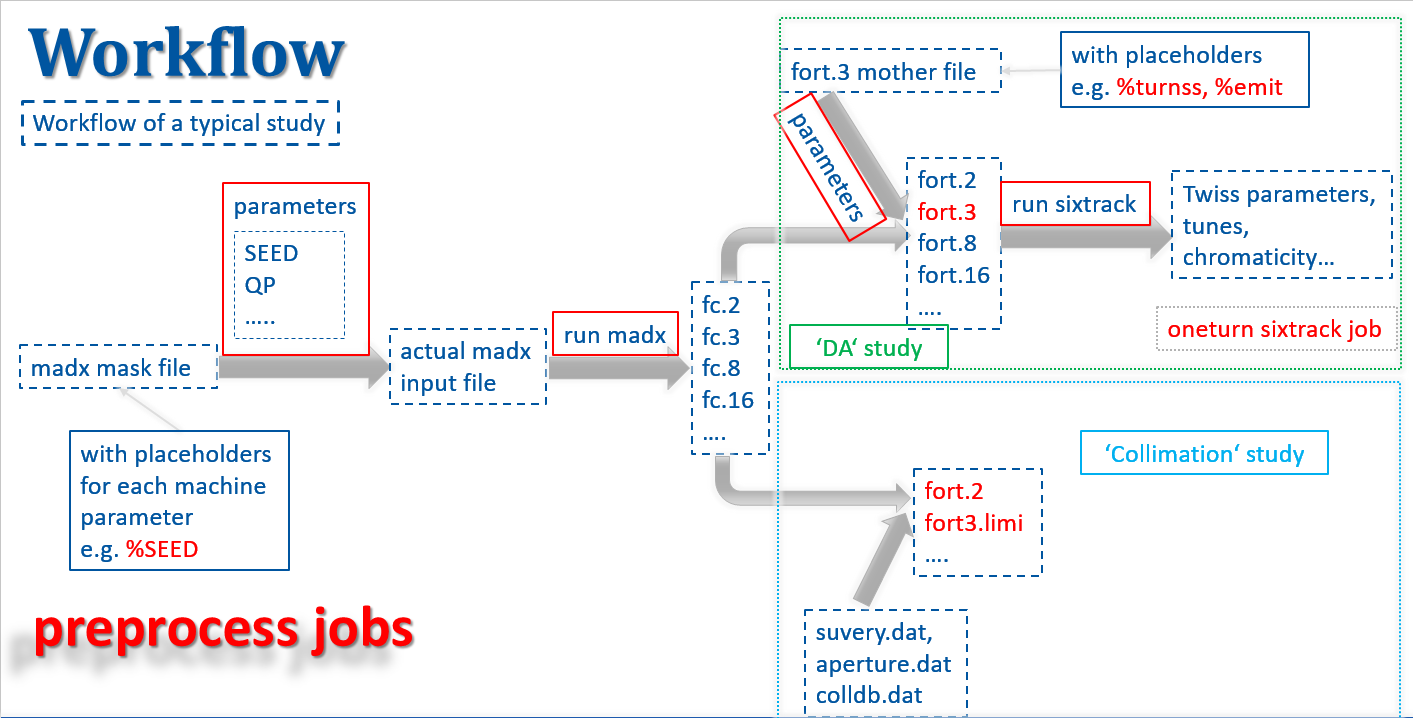
\includegraphics[width=17cm]{preprocess.png}
\caption{The workflow of preprocess job}
\label{fig1}
\centering
\end{figure}

The program will create the actual madx input file and execute madx to generate files for sixtrack jobs. In general, they will be 'fc.2', 'fc.3', 'fc.8', 'fc.16'. If the user is working on dynamic aperture (DA) study, the one-turn sixtrack job is needed to get the twiss-parameters. If the user is working on collimation study, an additional step to merge aperture model onto fort.2 is needed.

Note that the oneturn step will disappear once the new DIST block in sixtrack is done(which is ongoing), and also the additional step for merging aperture model will disappear once aperture markers and aperture offsets can be consistently generated by MADX.


\paragraph{sixtrack job}~

After the preprocess jobs are finished, the user can begin to prepare and submit sixtrack jobs. The workflow of sixtrack job is shown in Figure \ref{fig2}, the job will start from a template file 'fort.3' with some placeholders. The program will replace the placeholders with the corresponding values defined in config.py to generate the actual input file 'fort.3', the execute sixtrack to generate the required results.
\begin{figure}[h]
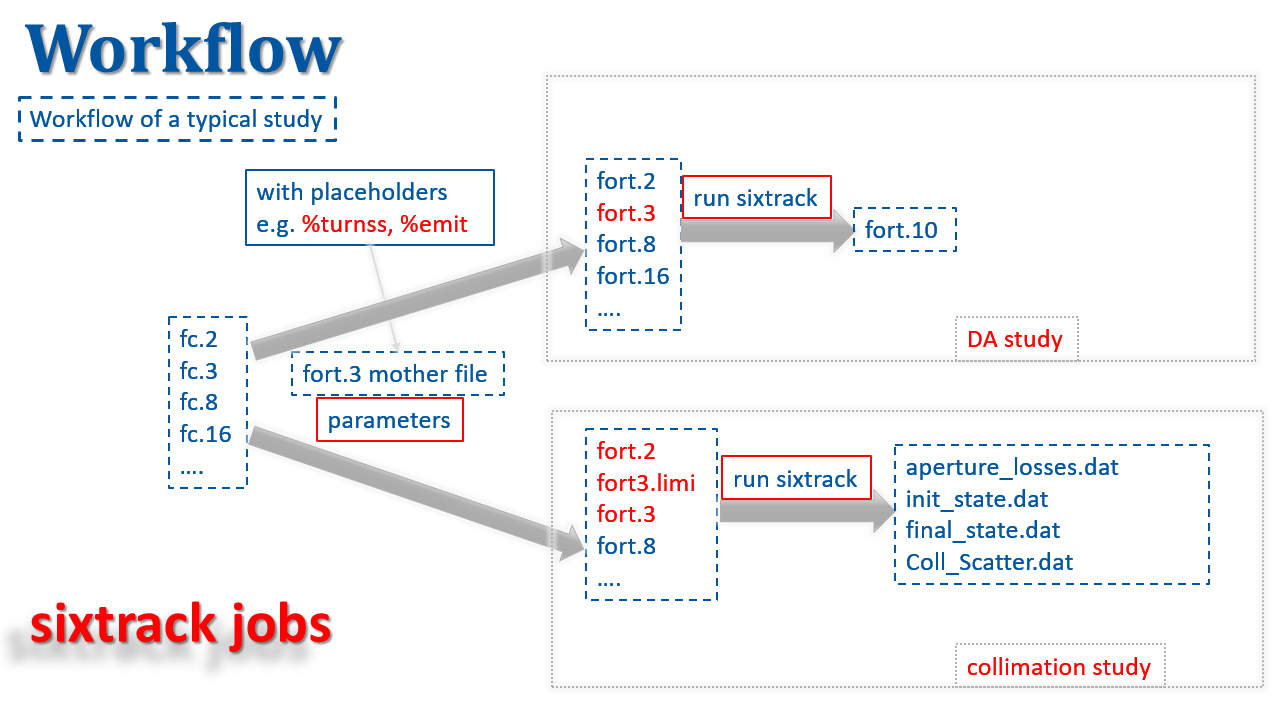
\includegraphics[width=17cm]{sixtrack.png}
\caption{The workflow of sixtrack job}
\label{fig2}
\centering
\end{figure}

The detailed command to manage these steps will introduce in the next chapter.

\paragraph{parameter scan}~

For both madx job and sixtrack job, the user can scan the paratemeter conveniently in pysixdesk. Define the paratemeters for scan as list, and by default the program will generate all the studies over a Cartesian grid. For example, if the user is working on DA study and going to do the phase space scan:

\begin{lstlisting}
...
self.sixtrack_params['amp'] = [(8,10), (10, 12)]
self.sixtrack_params['kang'] = [1,2]
...
\end{lstlisting}

And the program will insert 4 new lines in the table sixtrack\_wu with:
\begin{lstlisting}
(...(8,10), 1...), (...(8,10), 2...), (...(10,12), 1...), (...(10,12), 2...)
\end{lstlisting}
The user can also use a custom algorithm to do the scan except for Cartesian grid, just override the 'custom\_product\_preprocess' and 'custom\_product\_sixtrack' method with a new algorithm in the config.py file.

\section{Database}

In pySixDesk, sqlite3 and mysql are employed as the main databases to store the data. sqlite3 is the local file-based db, and mysql is the server-based db. For sqlite3 database, it will sit in your study path with an unified name \textbf{data.db}, and for mysql database, we use the DB-On-Demand server which is managed by CERN IT.
  To connect to mysql, the username, password, host, port are needed at least. For security reason, the \textbf{config.py} doesn't hold these information, the user should prepare a config file \textbf{.my.cnf} under the home directory \textbf{(\$HOME)} which contains the information, it looks like:
\begin{lstlisting}
[client]
user = test1
password = test
host = 127.0.0.1
port = 3306
\end{lstlisting}

\paragraph{Tables}~

There are several tables for a study in the database. 
\begin{lstlisting}[language=Python]
boinc_vars # for boinc variable
env # for some general valriables 
templates # template files, such as *.mask, fort.3
preprocess_wu # parameters for preprocess job
preprocess_task # records for all the preprocess tasks (each submission)
oneturn_sixtrack_wu # parameters for one-turn parameters
sixtrack_wu # parameters for sixtrack job
sixtrack_task # records for all the sixtrack task (each submission)

oneturn_sixtrack_results # results of one turn sixtrack jobs
six_results # results of actual sixtrack jobs
#some general info of the tracking
init_state
final_state
aperture_losses
#results of collimation study
collimation_losses
\end{lstlisting}
The detailed description of the tables can be found in \url{https://github.com/SixTrack/pysixdesk/blob/master/doc/Table.md}

\section{Special features}

There are also some special features in pysixdesk:
\begin{enumerate}
\item submit from local computer. Due to HTCondor have the spooling ability, so the user can submit jobs from a local computer. To use this feature, the user should setup kerberos and HTCondor on a local computer at first. Here is a sample instruction:
\url{https://twiki.cern.ch/twiki/bin/view/ABPComputing/LxbatchHTCondor}. 

Note that the user should submit jobs with '-spool' option from a local computer.

\item group the jobs. pysixdesk could group the jobs by the given parameter. e.g. group by amplitude, then each group will have all scanned values of amplitude but same values of other parameters. And a group will be submitted to one HTCondor node.

\item prolong tracking. pysixdesk could prolong the tracking with checkpoint/restart feature. There are three flag in config.py to switch this feature, 'self.checkpoint\_restart = False', 'self.first\_turn=1', 'self.last\_turn=100'. If checkpoint\_restart is set to True, the program will find the checkpoint files (if exist) and prolong the complete job. 

Note that the user should make sure the sixtrack executable in use is compiled with the CR option.
\end{enumerate}

\section{Tests}

Below is a scalability test result for different databases. The test condition: 300 preprocess jobs, 30000 sixtrackjobs. All operations were done on CERN lxplus and all jobs were submitted to HTCondor.
\begin{table}[h]
    \caption{Scalability tests for these two databases.}
    \label{T-ExtRou}
    \centering
    \renewcommand{\arraystretch}{1.5}
    \begin{tabular}{|l|l|l|}
        \hline
        \rowcolor{blue!30}
        \textbf{Action/DB} & \textbf{Sqlite3} & \textbf{Mysql} \\
        \hline
        \texttt{setup DB}  & 5s & 11s \\
        \hline
        \texttt{prepare preprocess}  & 1s & 1s \\
        \hline
        \texttt{submit}   & 6s    & 27s \\
        \hline
        \texttt{collection}   & 120s   & - \\
        \hline
        \texttt{prepare sixtrack}  & 240s & 128s \\
        \hline
        \texttt{submit}   & 435s    & 294s \\
        \hline
        \texttt{collection}   & ~3h   & - \\
        \hline
    \end{tabular}
\end{table}

Where '-' represent no need.
Note that if the user select mysql and submit jobs to BOINC, the collection process is still needed. For the moment, the volunteer computers can't access to the mysql server directly.

%\subsection{Command Line Arguments} \label{sec:cmdarg}
%
%SixTrack does not require any command line arguments, but can optionally take the file name for the main input file as well as the geometry file as the first and second argument, respectively.
%See also Sections~\ref{InFiles} and~\ref{ProVer}.
%
%\bigskip
%\noindent In addition, SixTrack can echo the version number and exit with the following flags:
%\begin{itemize}
%    \item[\texttt{-v}] Echo program name and version as a single line, and exit.
%    \item[\texttt{-V}] Echo program name, version, release date, and git hash on four lines, and exit.
%    \item[\texttt{-nv}] Echo the numerical version as an integer, and exit,
%\end{itemize}
